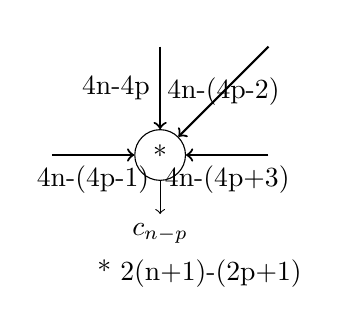
\begin{tikzpicture}[scale=0.5]

    \tikzset{nodestyle/.style={draw,shape=circle}}
    \node (p2) at ( 3, 0) {};
   \node(p33) at (7,-3) {* 2(n+1)-(2p+1)};
    \node[nodestyle] (p3) at (6, 0) {*};
    \node (p4) at ( 9, 0) {};

    \node (p8) at ( 9, 3) {};
    \node (p9) at ( 6, 3) {};

    \begin{scope}[every path/.style={->,thick}]
        \draw (p2) -- (p3)node[midway,below]{4n-(4p-1)}; 
        \draw (p4) -- (p3)node[midway,below]{4n-(4p+3)};

        \draw (p9) -- (p3)node[midway,left]{4n-4p};
        \draw (p8) -- (p3)node[midway]{4n-(4p-2)};

    \end{scope} 
    \node (c2) at ( 6, -2) {$c_{n-p}$};

        \draw[->] (p3) -- (c2);
\end{tikzpicture}
